\documentclass[12pt, twoside]{article}
\usepackage[letterpaper, margin=1in, headsep=0.5in]{geometry}
\usepackage[english]{babel}
\usepackage[utf8]{inputenc}
\usepackage{amsmath}
\usepackage{amsfonts}
\usepackage{amssymb}
\usepackage{tikz}
%\usetikzlibrary{quotes, angles}

\usepackage{graphicx}
\usepackage{enumitem}
\usepackage{multicol}

\usepackage{fancyhdr}
\pagestyle{fancy}
\fancyhf{}
\renewcommand{\headrulewidth}{0pt} % disable the underline of the header

\fancyhead[RE]{\thepage}
\fancyhead[RO]{\thepage \\ Name: \hspace{3cm}}
\fancyhead[L]{BECA / Dr. Huson / 10th Grade Geometry\\* Unit 7: Analytic Geometry Review\\25 February 2019}

\begin{document}
\subsubsection*{7-14 Triangle midlines and similar triangles}
  \begin{enumerate}

    \item Triangle $ADE$ is drawn with $\overline{BC} \parallel \overline{DE}$, as shown. Given $AB=5$, $BC=7$, $AC=8$, and $BD=5$. \\[0.25cm] Find $CE$, $AE$, and $DE$. \vspace{1cm}
    \begin{center}
      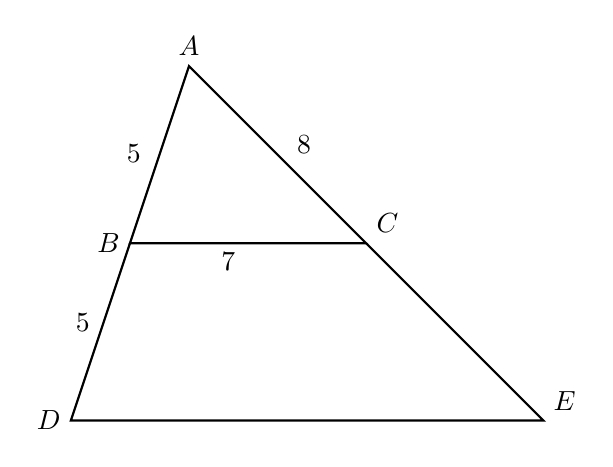
\begin{tikzpicture}[scale=0.5]
        \draw [thick]
        (0.5,1.5)node[left]{$B$}--
        (6.5,1.5)node[above right]{$C$}--
        (2,6)node[above]{$A$}--cycle;
        \draw [thick]
        (0.5,1.5)--
        (-1,-3)node[left]{$D$}--
        (11,-3)node[above right]{$E$}--(6.5,1.5);
        \node at (3,1.5)[below]{$7$};
        \node at (4.5, 4)[right]{$8$};
        \node at (0.6, 3.3)[above]{$5$};
        \node at (-0.7, -1)[above]{$5$};
      \end{tikzpicture}
    \end{center} \vspace{1cm}

    \item Triangle $ABC$ is dilated with a factor of $k=2$ centered at $A$, yielding $\triangle ADE$, as shown. Given $AB=10$, $BC=12$, and $AC=14$. \\[0.25cm] Find $AD$, $AE$, and $DE$. \vspace{1cm}
    \begin{center}
        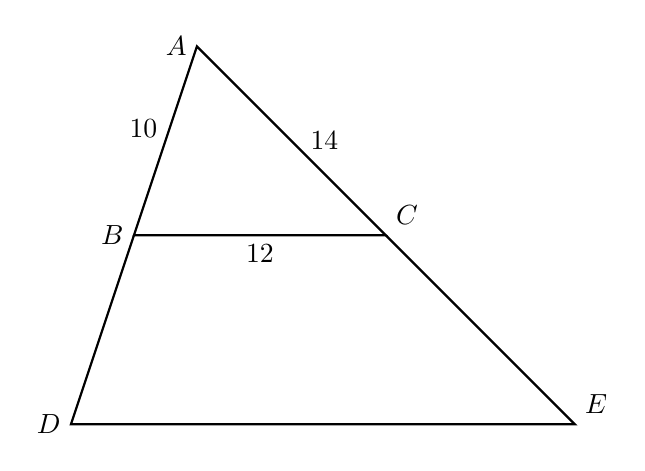
\begin{tikzpicture}[scale=0.4]
          \draw [thick]
          (0,0)node[left]{$B$}--
          (8,0)node[above right]{$C$}--
          (2,6)node[left]{$A$}--cycle;
          \draw [thick]
          (0,0)--
          (-2,-6)node[left]{$D$}--
          (14,-6)node[above right]{$E$}--(8,0);
          \node at (4,0)[below]{$12$};
          \node at (5.3, 3)[right]{$14$};
          \node at (0.3, 2.8)[above]{$10$};
        \end{tikzpicture}
      \end{center}

  \newpage

   \item Given $\triangle ABP$ and $\triangle JKP$ as shown below. $\overline{AB} \parallel \overline{JK}$. $AP=5.7$, $JP=11.4$, and $JK=14.8$. Find $AB$.\\[0.5cm]
     \begin{tikzpicture}[scale=1.4]
         \draw [thick]
           (0.25,-1)node[right]{$B$}--
           (-0.5,2)node[left]{$K$}--
           (4,0)node[right]{$J$}--
           (0,0)node[above right]{$P$}--
           (-2,0)node[left]{$A$}--cycle;
       \end{tikzpicture}




  \end{enumerate}
\end{document}
